\section{Reconstruction and Scalability of Coordinate Descent}
%\textbf{Coordinate Descent comparison to CLEAN reconstruction}
In this section, we compare the Coordinate Descent reconstruction with CLEAN on simulated MeerKAT data, and compare the runtime complexity of the two approaches on a real-world MeerKAT observation. We show that Coordinate Descent reconstructs the image by only computing a few columns of the Fourier Transform Matrix $F^{-1}$, and investigate if this approach reduces the runtime complexity on the large scale reconstruction problems of MeerKAT.

The real world MeerKAT data were calibrated and averaged down to reduce its size to 88 Gigabytes. The raw, uncalibrated data ranges between 500 and 1000 Gigabytes. Data on this scale requires a mature pipeline for reading and image reconstruction. Within the time limit of this project, only a reconstruction with the WSCLEAN\cite{offringa2014wsclean} pipeline was possible.

The simulations were created with the Meqtrees software package. Two simulations which contain roughly (size of Visibilities) perfectly calibrated Visibilities were created. Compared to real-world observations, the two simulated data sets are small and not representative of the real data volume. Also, more realistic simulations which contain pointing errors, calibration errors, and thermal noise are out of scope for this project. The simulations are used to isolate the two fundamental issues in radio interferometer image reconstruction: Non-uniform sampling and incomplete measurements.

\subsection{Imaging on Simulated Data}
We compare the reconstruction of Coordinate Descent and CLEAN on two simulated observations. The first observation contains two point sources, on which we show that Coordinate Descent is able to locate the sources below the accuracy limit of the instrument. The second observation contains point and Gaussian sources, on which we show that Coordinate Descent better captures the intensity profile of extended emissions. Also, we look at the shortcomings of the proof-of-concept implementations in terms of reconstruction quality and runtime. We use the CLEAN implementation of CASA in this section. CASA is an established software framework for radio interferometer image reconstruction and was already used in a previous project.

\begin{figure}[h]
	\centering
	\begin{subfigure}[b]{0.4\linewidth}
		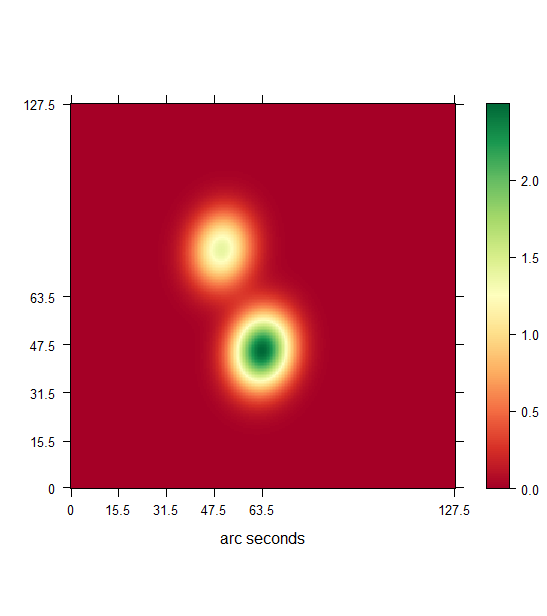
\includegraphics[width=\linewidth]{./chapters/20.results/points/tCLEAN.png}
		\caption{CLEAN reconstruction.}
		\label{results:points:tclean}
	\end{subfigure}
	\begin{subfigure}[b]{0.4\linewidth}
		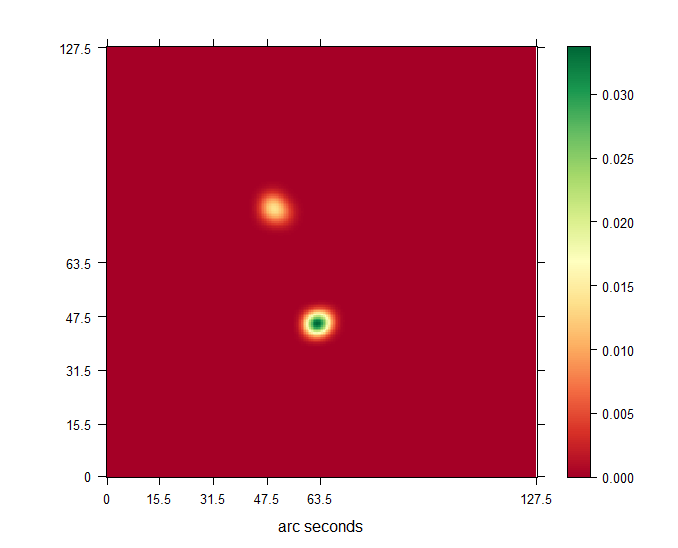
\includegraphics[width=\linewidth]{./chapters/20.results/points/cd.png}
		\caption{Coordinate Descent reconstruction.}
		\label{results:points:cd}
	\end{subfigure}
	
	\caption{Image reconstruction of two point sources.}
	\label{results:point}
\end{figure}

We used CASA's default parameters for CLEAN, except for the maximum number of CLEAN iterations, which we set to 250. The proof-of-concept Coordinate Descent implementation has three parameters to tune: Number of iterations, the number of starlet layers $J$, and the regularization parameter $\lambda$. The first two parameter could be estimated by the reconstruction algorithm itself. In this implementation, it was left to the user. For the two simulations the Coordinate Descent parameters were chosen:
\begin{itemize}
	\item Two Point sources: 4 full iterations, $J=3$, $\lambda=0.1$
	\item Mixed sources: 4 full iterations, $J=7$, $\lambda=0.1$
\end{itemize}

In figure \ref{results:point} shows an image of the Coordinate Descent and CLEAN reconstruction. Figure \ref{results:points:contour} shows the intensity profile of both reconstructions compared with the ground truth. Note that figure \ref{results:points:contour} has a logarithmic y axis. The reconstructions differ in two notable ways: The peak intensity of the source, and how much each algorithm spreads the point source. 

\textit{Spread}: CLEAN reconstructs a convolved version of the true image. CLEAN locates the two peaks in figure \ref{results:points:contour}, but convolves the point source with a Gaussian function. CLEAN reconstructs two Gaussian functions with same peak as the point source. The Gaussian represents the accuracy of the instrument. With compressed sensing, we try to reconstruct the observed image above the accuracy of the instrument. In the intensity profile \ref{results:points:contour}, Coordinate Descent reconstructs two narrow gaussian-like peaks, essentially super-resolving the image. However, note that the total intensity is a fraction of the original peaks.

\textit{Intensity:} [Total Flux] The reconstructions differ in intensity. The figure \ref{results:points:contour} shows the intensity profile of the two reconstructions. Note the $y$ axis is on a logarithmic scale. Also note that Coordinate Descent has shifted the smaller peak by a pixel in its reconstruction. [Total flux correct in CD?]

\begin{figure}[h]
	\centering
	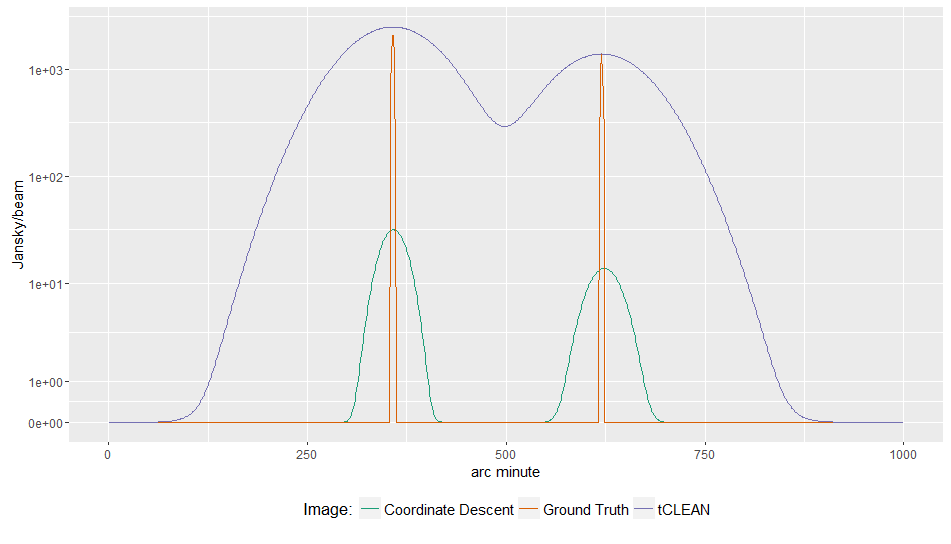
\includegraphics[width=0.8\linewidth]{./chapters/20.results/points/line.png}
	\caption{Intensity profile of the two point sources.}
	\label{results:points:contour}
\end{figure}

The difference in intensity becomes more apparent with extended emissions. Figure \ref{results:mixed} shows Coordinate Descent and tCLEAN on the simulation with mixed sources. Again the two reconstructions arrive at different intensities. The gaussian emissions are reconstructed with a higher intensity than Coordinate Descent.

\begin{figure}[h]
	\centering
	\begin{subfigure}[b]{0.4\linewidth}
		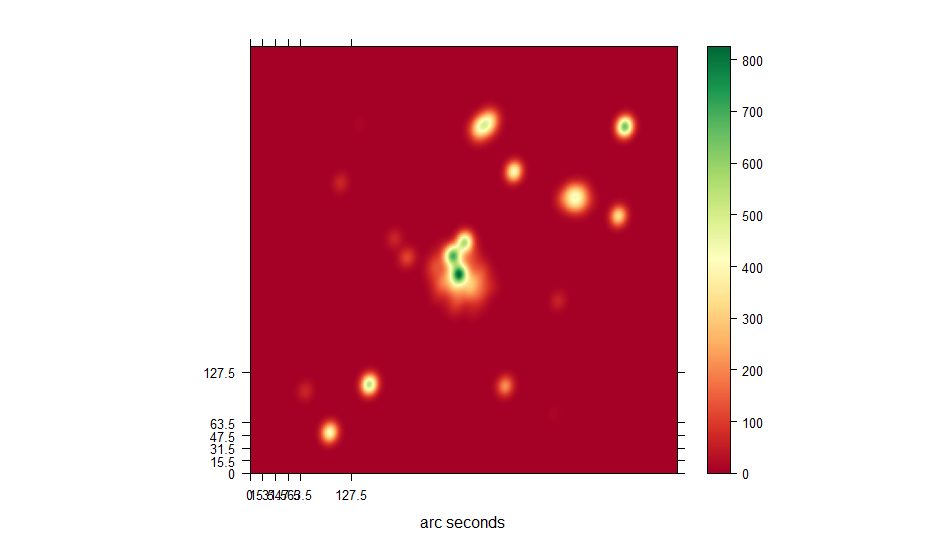
\includegraphics[width=\linewidth]{./chapters/20.results/mixed/mixed_tclean.png}
		\caption{tclean reconstruction}
		\label{results:mixed:tclean}
	\end{subfigure}
	\begin{subfigure}[b]{0.4\linewidth}
		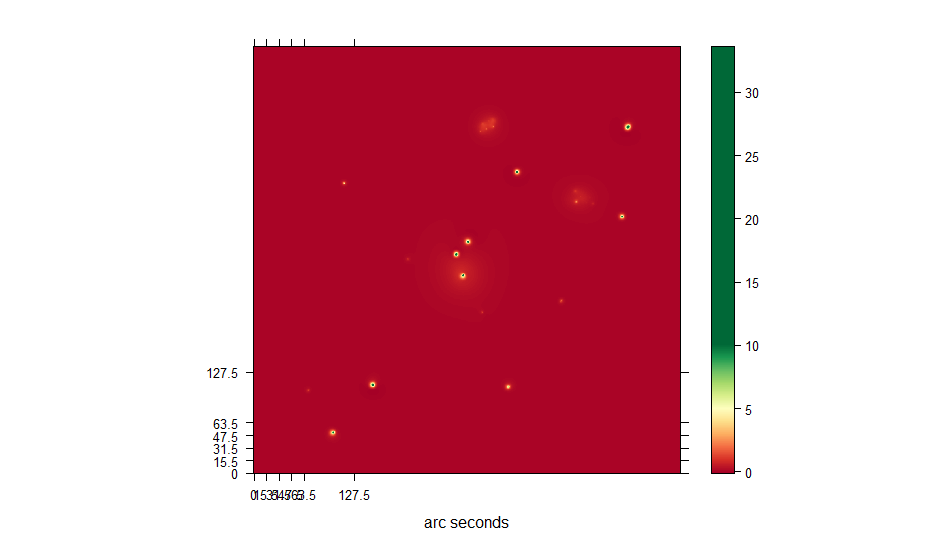
\includegraphics[width=\linewidth]{./chapters/20.results/mixed/mixed_cd.png}
		\caption{Coordinate Descent Reconstruction}
		\label{results:mixed:cd}
	\end{subfigure}
	\caption{Reconstruction on mixed sources}
	\label{results:mixed}
\end{figure}

With starlets, coordinate descent has a representation for extended emissions. Looking at the intensity profile of an extended emisions \ref{}, we see Coordiante Descent coming closer to the true intensity. Although in the four iterations,  [it still had a considerable margin on error]. 

Total flux constraint, $\lambda$ for different starlet layers like in \cite{girard2015sparse}

Coordinate Descent did not reconstruct all point sources. How many starlets are non-zero is the major point for runtime. It depends on how many areas of the image are non-zero. Starlet has a representation for extended emission, how many starlets are needed for modelling is hard.

Runtime problems
7000 non-zero starlets, 


\subsection{Scalability estimate of CLEAN and Coordinate Descent}
%\begin{figure}[h]
%	\centering
%	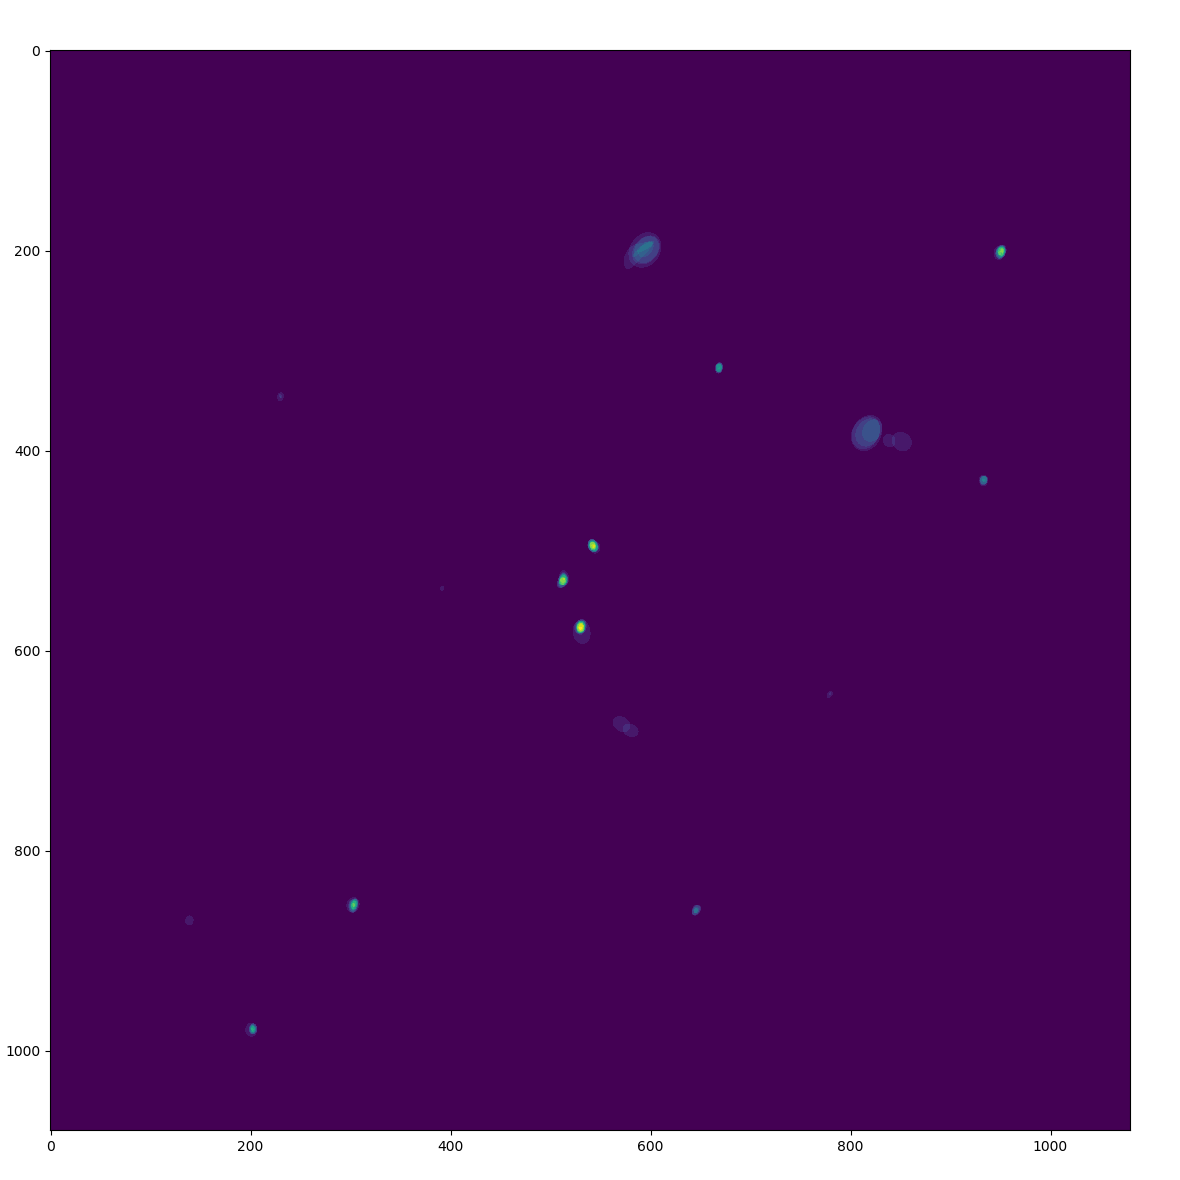
\includegraphics[width=0.5\linewidth]{./chapters/05.algorithms/sim00/full_cache_debug.png}
%	\caption{Pixels used to reconstruct the image}
%	\label{results:pixels:used}
%\end{figure}
In this section, we first discuss the runtime complexity of Coordinate Descent and CLEAN. We compare the runtime complexity on a real MeerKAT observation and come to the conclusion, that the Major Cycle Architecture leads to a lower runtime complexity. 

 depends too heavily on the


Pinning down the precise runtime of Coordinate Descent is difficult. As mentioned in section \ref{cd}, Coordinate Descent has lose convergence guarantees in theory, but works well in practice with heuristics. However, these heuristics complicate the runtime analysis of Coordinate Descent. How well the active set heuristic performs on an average case is a difficult analysis.

Furthermore the current implementation can potentially be improved with other heuristics. In this section, we account for potential heuristics by looking at the best case runtime complexity of Coordinate Descent. We compare it to the complexity of CLEAN on a real MeerKAT observation. It turns out that CLEAN and the Major Cycle architecture eadd to a lower runtime complexity on large datasets.

\subsubsection{Runtime complexity of Coordinate Descent}
The runtime complexity of Coordinate Descent depends largely on the number of Visibilities $M$ and the number of non-zero starlets $S$. The number and location of the $S$ non-zero starlets are generally not known. However, we created a heuristic which finds likely non-zero starlet components. In a realistic setting, the heuristic will have found more than $S$ likely non-zero starlets. For the best case scenario, we assume an oracle performance heuristic: It finds the location and number of the $S$ non-zero starlet components in constant time ($O(1)$). Coordinate Descent therefore has to find the value of the $S$ non-zero starlet components, which takes three separate operations: creating the columns of $F^{-1}$, calculating the minima for each single component, and calculating the starlet layers:

\begin{alignat*}{1}
\text{creating} \:S\: \text{columns of}\: F^{-1} &: S*3M\\
\text{locating} \:S\: \text{minima of} \:S\: \text{parabolas} &: S*8M\\
\text{calculating} \:J\: \text{Starlet layers} &: J * 2M
\end{alignat*}

We assume we have enough memory to cache the columns of $F^{-1}$ and only need to calculate them once. Coordinate Descent arrives at the correct result in $I_{CD}$ iterations. Therefore we arrive at the runtime complexity of \eqref{results:cd:omega}.

\begin{equation}\label{results:cd:omega}
CD(I_{CD}, M, S, J) = S*3M + I_{CD} * [S * 8M + J * 2M]
\end{equation}

Note that the runtime of Coordinate Descent is independent of the number of pixels. The only image related parameter in \eqref{results:cd:omega} is $J$, the number of starlet layers. The largest starlet layer represents the largest possible structure in the image, which is given by the instrument and the image resolution (pixels per arc-second). The runtime only depends indirectly on the image resolution, not the total number of pixels.

Also note the term iterating over the $S$ non-zero starlets, $ I_{CD} * [S * 8M +\ldots]$. As it turns out, this is the Achilles heel of the algorithm. MeerKAT observations contain a very large amount of Visibilities $M$ and a large amount of distinct structures, which leads to a large $S$ (each point source needs at least one non-zero component to be represented). 

\subsubsection{Runtime complexity of CLEAN}
We look at CLEAN reconstructions which use the non-uniform FFT with $w$-stacking. The runtime of a single Major cycle depends on the non-uniform FFT with $w$-stacking and the number of CLEAN deconvolutions. The number $N$ denotes the number of pixels (for example $512^2$).

\begin{alignat*}{1}
	\text{non-uniform FFT} &: M + 2N*ld(2N)\\
	\text{non-uniform FFT with} \:w\text{-stacking} &:M + W*(2N*ld(2N) + 2N) + N*ld(N)\\
	I_{CLEAN}\: \text{deconvolutions} &: I_{CLEAN}*2N
\end{alignat*}

The overall complexity shown in \eqref{results:clean:o} can also be split into two parts: It depends on the number of Major on the number of Major Cycles $I_{Major}$ and the complexity of the non-uniform FFT, and $I_{Major}$ times the CLEAN deconvolutions. 

\begin{equation}\label{results:clean:o}
\begin{aligned}
 CLEAN(I_{Major}, I_{CLEAN}, M, N,  W) =\: &I_{Major} * 2 * [M + W*(2N log 2N + 2N) + N log N]\\
+ &I_{Major} * [I_{CLEAN}*2N]
\end{aligned}
\end{equation}

Notice that the number of CLEAN deconvolutions $I_{CLEAN}$ depends on the image content, similar the number of non-zero starlets $S$ for Coordinate Descent. Here however, it multiplies with the number of pixels $N$ instead of the number of Visibilities $M$. In a sense, the major cycle tries to reduce the runtime complexity of handling the image content by calculating the non-uniform FFT. If the difference is large enough $N \ll M$, then the Major Cycle will end up with a smaller overall runtime.

\subsubsection{Runtime complexity estimate on MeerKAT data}
The MeerKAT observation contains approximately 540 channels with 4 million calibrated Visibilities each. After calibration, MeerKAT data is typically averaged over frequency and time to reduce its disk space. There are no strict rules on how to chose the image resolution and number of pixels. An initial WSCLEAN reconstruction was preformed with:
\begin{itemize}
	\item Visibilities: $M=2.19e^9$
	\item $w$-stacks: $W = 128$
	\item Pixels: $N = 8192^2$
	\item Maximum number of CLEAN iterations: $I_{CLEAN} = 35'000$
\end{itemize}

Let us use these numbers and compare the complexity of WSCLEAN \eqref{results:clean:o} with Coordinate Descent \eqref{results:cd:omega}. There are three values left to define: The number of Major Cycles $I_{Major}$ for CLEAN, and for Coordinate Descent the  number of non-zero starlets $S$, iterations $I_{CD}$, and starlet levels $J$. CLEAN reconstructions tend to use around five Major Cycles. For the first estimate, we make assumptions in favour of Coordinate Descent and set $I_{Major} = 10$. 10 Major Cycles is what a compressed sensing reconstruction needed to converge on simulated data \cite{pratley2018fast}. For Coordinate Descent we set $J = 10$, which lets the largest starlet span $5*2^{10} = 5120$ pixels, and an area of 136 arc-minutes. More than enough to capture the largest structures in the image. We compare the relative speedup of Coordinate Descent to CLEAN for different number of iterations $I_{CD}$ and non-zero starlets $S$. Table \ref{res:cd:table} shows the factor of how much Coordinate Descent is faster than CLEAN. With $S=500$ and $I_{CD} = 1$ iterations, Coordinate Descent is 4.69 times faster than CLEAN. 

\begin{table}[h!]
	\begin{center}
		\begin{tabular}{l|c|c|c} % <-- Alignments: 1st column left, 2nd middle and 3rd right, with vertical lines in between
			 & $I_{CD} = 1$ & $I_{CD} = 5$ &  $I_{CD} = 10$\\
			\hline
			$S=500$ & 4.69 &  1.19 & 0.62 \\
			$S=2500$ & 0.93 &  0.24 & 0.12 \\
			$S=5000$ & 0.47 &  0.12 & 0.06 \\
			$S=7500$ & 0.31 &  0.08 & 0.04 \\
		\end{tabular}
		\caption{Relative speed-up of Coordinate Descent compared to CLEAN. }
		\label{res:cd:table}
	\end{center}
\end{table}

[To put the numbers into perspective, Coordinate Descent used roughly 7000 non-zero starlets to reconstruct the image \ref{results:mixed:cd}, which is based on simulated data only containing Gaussian and point sources. When we look at the WSCLEAN reconstruction of the MeerKAT observation \ref{results:wsclean}, we see complex extended emissions and a large number of point sources. [Create a reconstruction with 7000 non-zero starlets]. We need more than 7000 non-zero starlets for an accurate reconstruction of the image \ref{results:wsclean}.]

\begin{figure}[h]
	\centering
	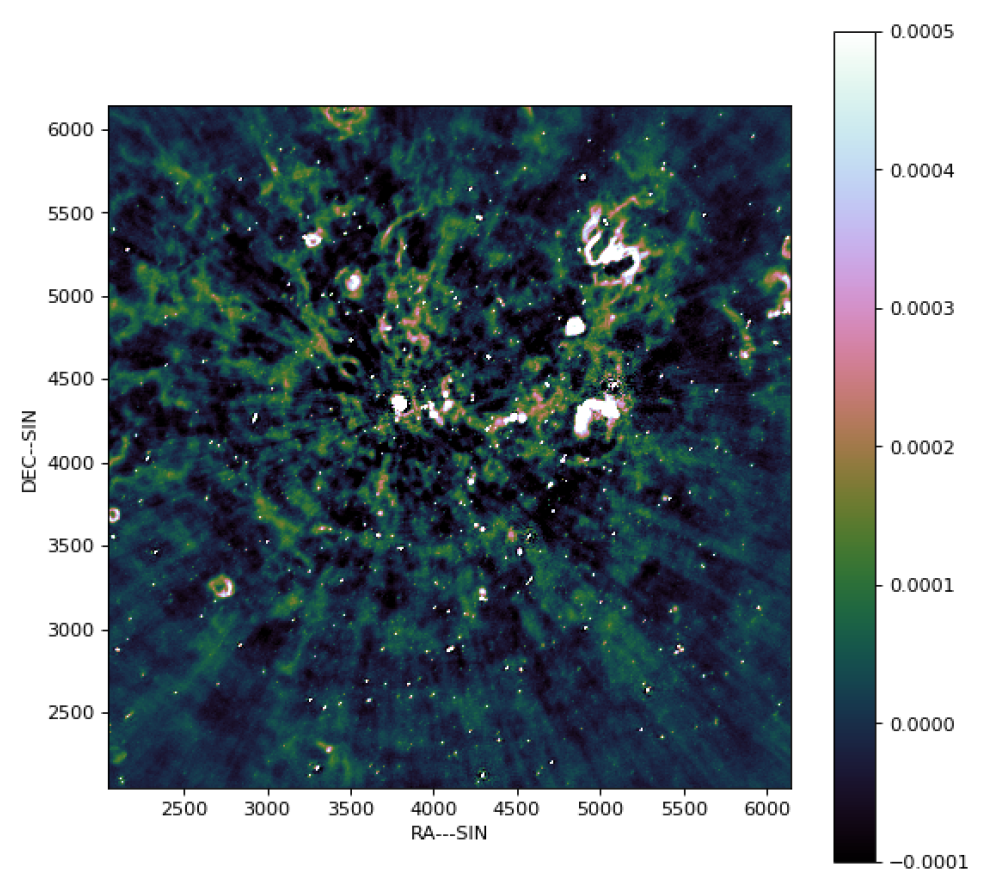
\includegraphics[width=0.6\linewidth]{./chapters/20.results/meerkat.png}
	\caption{WSCLEAN Reconstruction of the MeerKAT observation.}
	\label{results:wsclean}
\end{figure}

Since Coordinate Descent does not depend on the image size $N$, and the image size changes depending on the use case, one might imagine Coordinate Descent may be useful for very large image sizes. Sadly, this is not the case unless we create images with more pixels than Visibilities, which is not likely in the MeerKAT case. Let us quadruple each image dimension to $N=32000^2$, now we have two Visibilities for each pixel, and just for demonstration's sake reduce $J=5$ for Coordinate Descent. The results are shown in table \ref{res:cd:large:table}. Coordinate Descent is only competitive if it needs just one iteration to converge. Any advantage shrinks fast as soon as Coordinate Descent needs several iterations over all non-zero components $S$. How likely is it that Coordinate Descent just needs one iteration to converge?

\begin{table}[h!]
	\begin{center}
		\begin{tabular}{l|c|c|c} % <-- Alignments: 1st column left, 2nd middle and 3rd right, with vertical lines in between
			& $I_{CD} = 1$ & $I_{CD} = 5$ &  $I_{CD} = 10$\\
			\hline
			$S=500$ & 76.82 &  19.64 & 10.17 \\
			$S=2500$ & 15.38 &  3.39 & 2.03 \\
			$S=5000$ & 7.69 &  1.97 & 1.02 \\
			$S=7500$ & 5.13 &  1.31 & 0.68 \\
			$S=10000$ & 3.84 &  0.98 & 0.51 \\
			\hline
			$S=15000$ & 2.56 &  0.66 & 0.34 \\
			$S=20000$ & 1.92 &  0.49 & 0.25 \\
			$S=25000$ & 1.54 &  0.39 & 0.20 \\
		\end{tabular}
		\caption{Relative speed-up of Coordinate Descent compared to CLEAN with an image size of $N=32000^2$ and starlet levels $J=5$. }
		\label{res:cd:large:table}
	\end{center}
\end{table}

If the starlet components are independent of each other, Coordinate Descent finds the optimum value of each component in one iteration. As mentioned in section \ref{cd}, Starlets are an over-complete representation. Many many different starlet components explain the same data, which makes them dependent on each other and Coordinate Descent need several iterations to converge. The issue with Coordinate Descent's runtime complexity lies in the term $ I_{CD} * [S * 8M +\ldots]$ of \eqref{results:cd:omega}. Since $M$ is the largest number in the reconstruction problem, Coordinate Descent cannot afford many iterations. In a sense the Major Cycle architecture allows for more iterations, because it first converts the Visibilities $M$ into an image $N$, where $N \ll M$.

In other words, we could implement the Coordinate Descent Algorithm within a Major Cycle architecture, and we can afford more non-zero starlet components and more iterations for the same runtime complexity. This gets more obvious when we look at the memory footprint of Coordinate Descent: Each cached column of the Fourier Transform Matrix $F^{-1}$ contains $M$ elements. Assuming 32 bit floating point precision, a single column requires 8 gigabytes of memory. Caching several hundreds of columns is simply infeasible. However, if we would use the Major Cycle architecture, we may be able to use the FFT to calculate a single column, and do not need to cache it.

\subsection{Embracing the Major Cycle}


In this example, we over-estimated the runtime of CLEAN by setting the number of Major Cycles $I_{Major} = 10$, which is more in the area of current compressed sensing reconstructions. reconstructions. 

